\chapter{Indecșii Specifici OLTP și OLAP}
\label{sec:indecsi}

\section{Indecși OLTP (schema TickLy)}

\subsubsection{Pe tabelul TICKET și tabele copil}

\begin{itemize}
    \item \textbf{idx\_ticket\_client}, \textbf{idx\_ticket\_dept}, \textbf{idx\_ticket\_status}, \textbf{idx\_ticket\_prioritate}, \textbf{idx\_ticket\_categ}: B-tree pe coloanele FK, pentru join-uri și filtre
    \item \textbf{idx\_ticket\_data\_creare}: B-tree pe \texttt{data\_creare} — pentru filtre și sortări temporale
    \item \textbf{idx\_comm\_client\_tid}, \textbf{idx\_comm\_agent\_tid}: pe \texttt{comment\_client(ticket\_id)}, \texttt{comment\_agent(ticket\_id)} — listare comentarii per ticket
    \item \textbf{idx\_hist\_ticket\_tid}: pe \texttt{ticket\_history(ticket\_id)} — istoric evenimente per ticket
    \item \textbf{idx\_atasament\_ticket\_id}: pe \texttt{atasament(ticket\_id)}
    \item \textbf{idx\_ticket\_agent\_rev}: pe \texttt{ticket\_agent(agent\_id)} — tichete per agent
    \item \textbf{idx\_ticket\_tag\_rev}: pe \texttt{ticket\_tag(tag\_id)} — tichete per tag
\end{itemize}

\subsubsection{Indecși function-based (căutări case-insensitive)}

\begin{itemize}
    \item \textbf{idx\_client\_nume\_upper}, \textbf{idx\_client\_prenume\_upper}: pe \texttt{UPPER(nume)}, \texttt{UPPER(prenume)} în \texttt{client\_fizica}
    \item \textbf{idx\_juridic\_denumire\_upper}: pe \texttt{UPPER(denumire)} în \texttt{client\_juridica}
\end{itemize}

\section{Indecși OLAP (schema TickLy\_DW)}

\subsubsection{Pe tabelul de fapte și bridge}

\begin{itemize}
    \item \textbf{bidx\_fact\_status}: bitmap pe \texttt{fact\_ticket(status\_id)} — cardinalitate mică
    \item \textbf{bidx\_fact\_prioritate}: bitmap pe \texttt{fact\_ticket(prioritate\_id)}
    \item \textbf{bidx\_bridge\_tag}: bitmap pe \texttt{bridge\_ticket\_tag(tag\_key)}
    \item \textbf{idx\_bridge\_ticket\_id}: B-tree pe \texttt{bridge\_ticket\_tag(fact\_ticket\_id)} — cardinalitate mare
\end{itemize}

\subsubsection{Pe dimensiuni}

\begin{itemize}
    \item \textbf{idx\_dim\_client\_cnp}: B-tree pe \texttt{dim\_client(cnp)} — lookup și căutări pe CNP
\end{itemize}

\section{Cereri SQL și Plan de Execuție}

\begin{enumerate}
    \item \textbf{OLTP — index function-based pe \texttt{client\_fizica}}
    \begin{itemize}
        \item \textbf{1:} „Să se afișeze datele (identificator, CNP, nume, prenume) persoanelor fizice care au numele egal cu «RADU»”
    \end{itemize}

    \begin{verbatim}
        EXPLAIN PLAN FOR
        SELECT client_id, cnp, nume, prenume
        FROM TickLy.client_fizica
        WHERE UPPER(nume) = 'RADU';

        SELECT * FROM TABLE(DBMS_XPLAN.DISPLAY);
    \end{verbatim}

    \begin{figure}[H]
        \centering
        \begin{subfigure}[b]{0.48\textwidth}
            \centering
            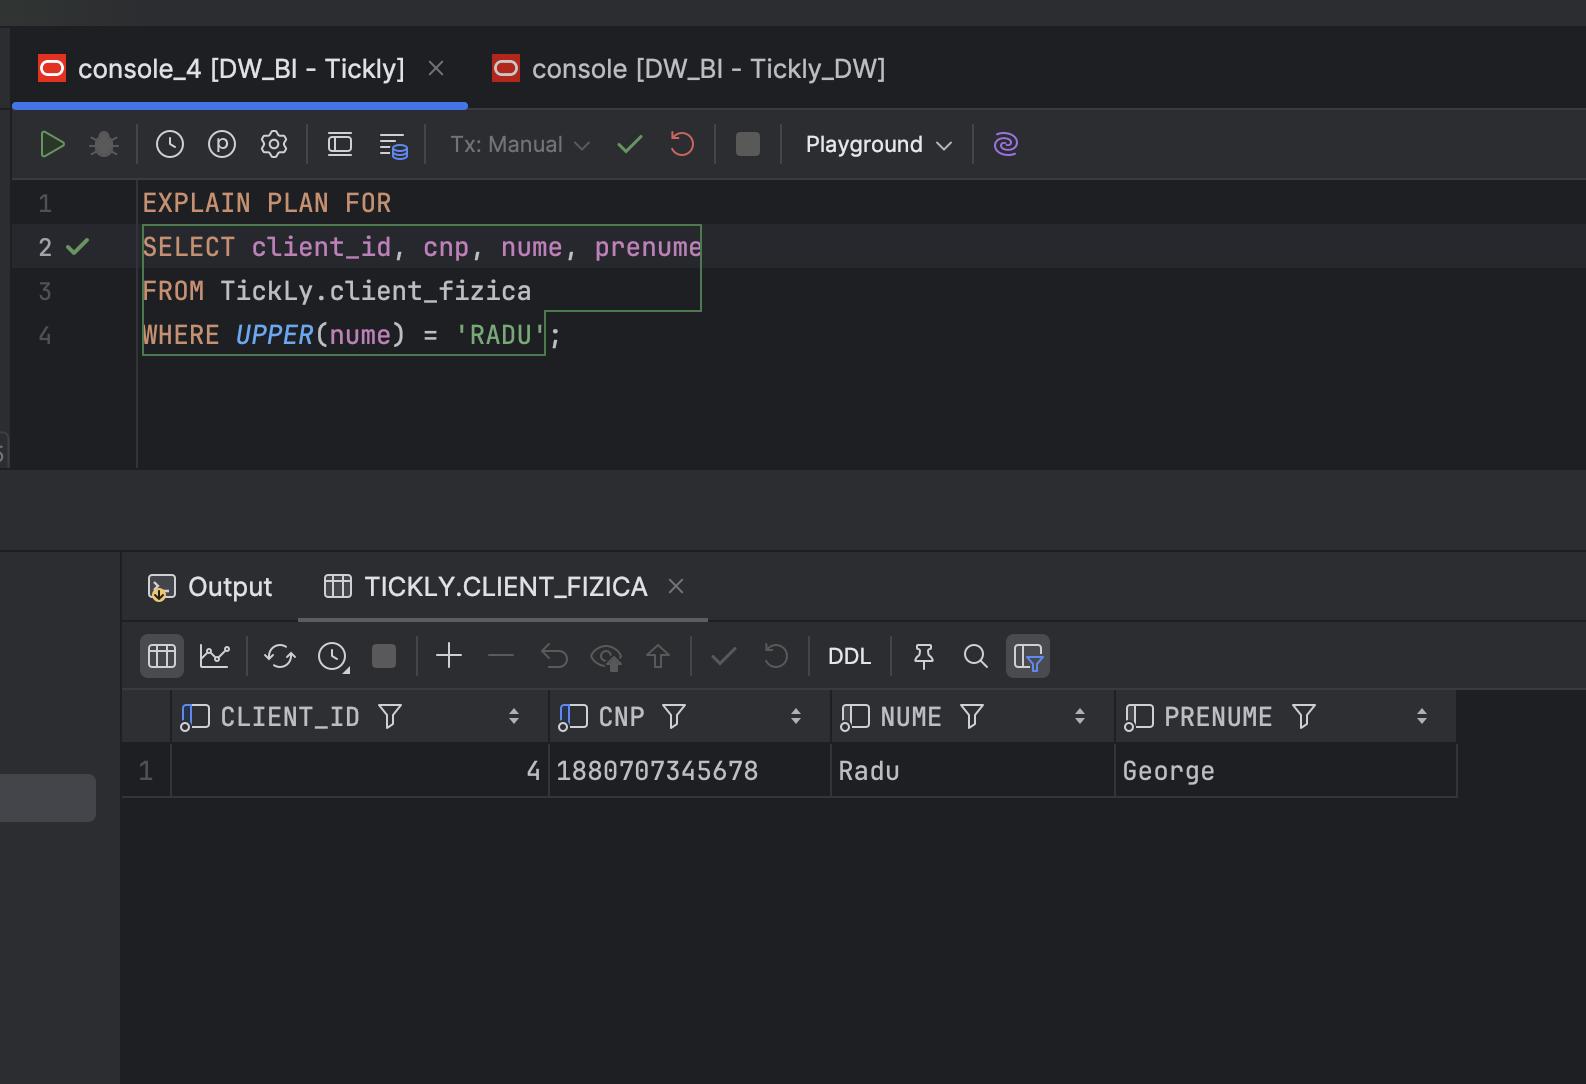
\includegraphics[width=\textwidth]{./assets/indexes/test_1.png}
            \caption{Rulare query 1}
            \label{fig:rulare_query_1}
        \end{subfigure}
        \hfill
        \begin{subfigure}[b]{0.48\textwidth}
            \centering
            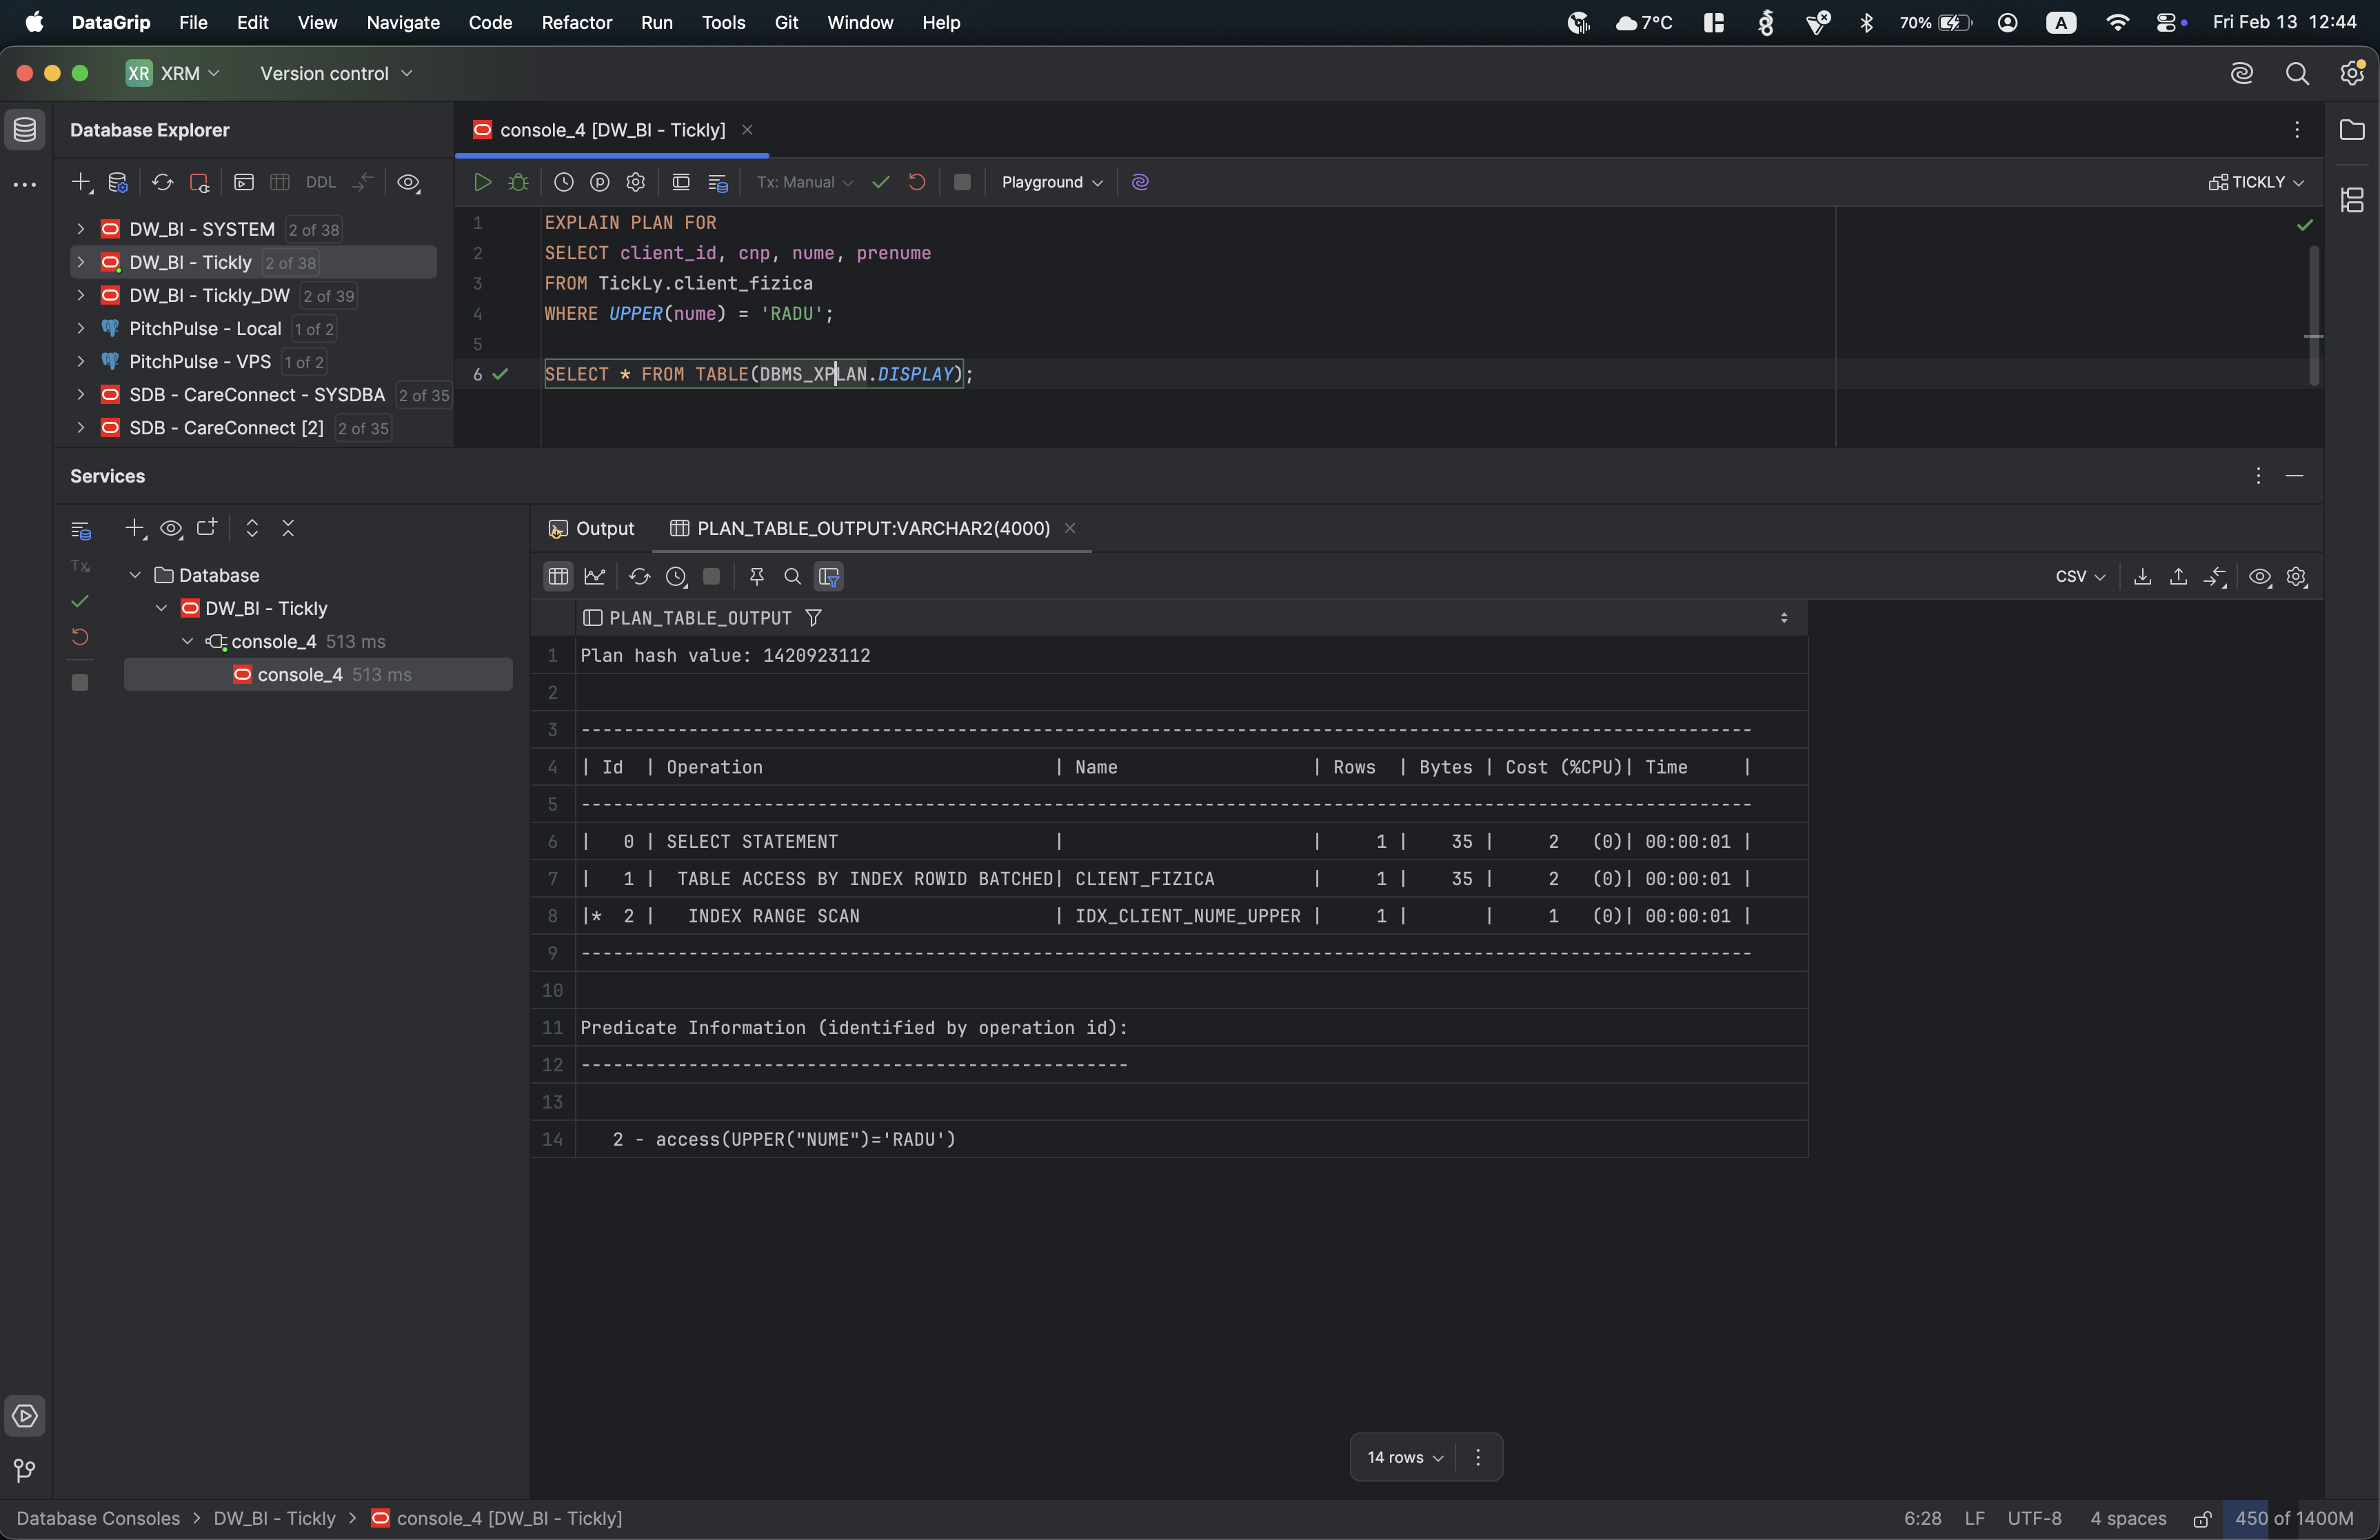
\includegraphics[width=\textwidth]{../../scripts/tests/assets/oltp_client_index_explain.png}
            \caption{Plan de execuție query 1}
            \label{fig:plan_executie_query_1}
        \end{subfigure}
        \caption{Analiză Query 1: Execuție și Plan}
        \label{fig:comparatie_query_1}
    \end{figure}

    \item \textbf{OLTP — index pe \texttt{ticket.data\_creare}}
    \begin{itemize}
        \item \textbf{2:} „Să se afișeze identificatorul, titlul, statusul și data creării pentru toate tichetele create în anul 2024, între luna februarie și luna decembrie.”
    \end{itemize}

    \begin{verbatim}
        EXPLAIN PLAN FOR
    SELECT ticket_id, titlu, status_id, data_creare
    FROM TickLy.ticket
    WHERE data_creare >= TO_DATE('01-FEB-2024', 'DD-MON-YYYY')
    AND data_creare < TO_DATE('01-DEC-2024', 'DD-MON-YYYY');

    SELECT * FROM TABLE(DBMS_XPLAN.DISPLAY);
    \end{verbatim}

    \begin{figure}[H]
        \centering
        \begin{subfigure}[b]{0.48\textwidth}
            \centering
            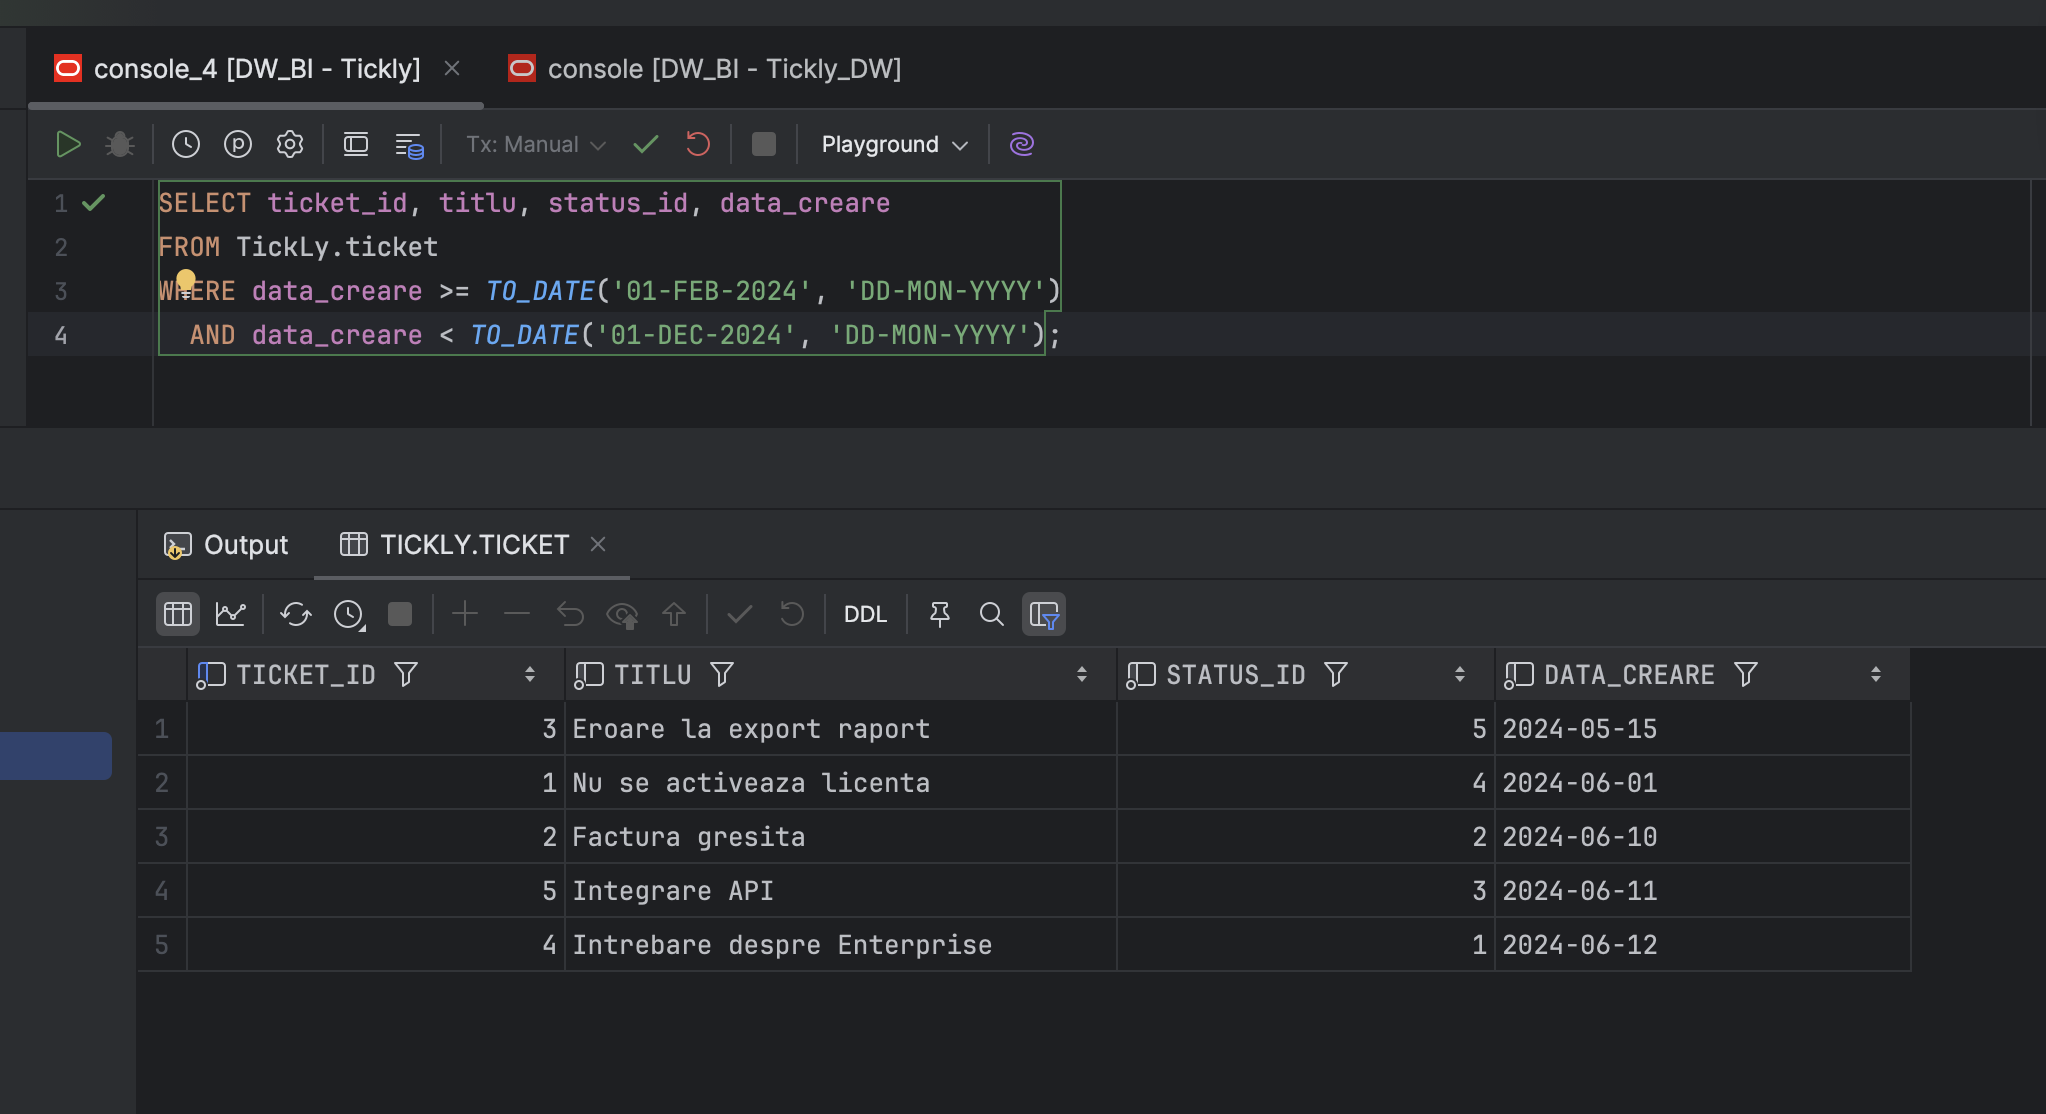
\includegraphics[width=\textwidth]{./assets/indexes/test_2.png}
            \caption{Rulare query 2}
            \label{fig:rulare_query_2}
        \end{subfigure}
        \hfill
        \begin{subfigure}[b]{0.48\textwidth}
            \centering
            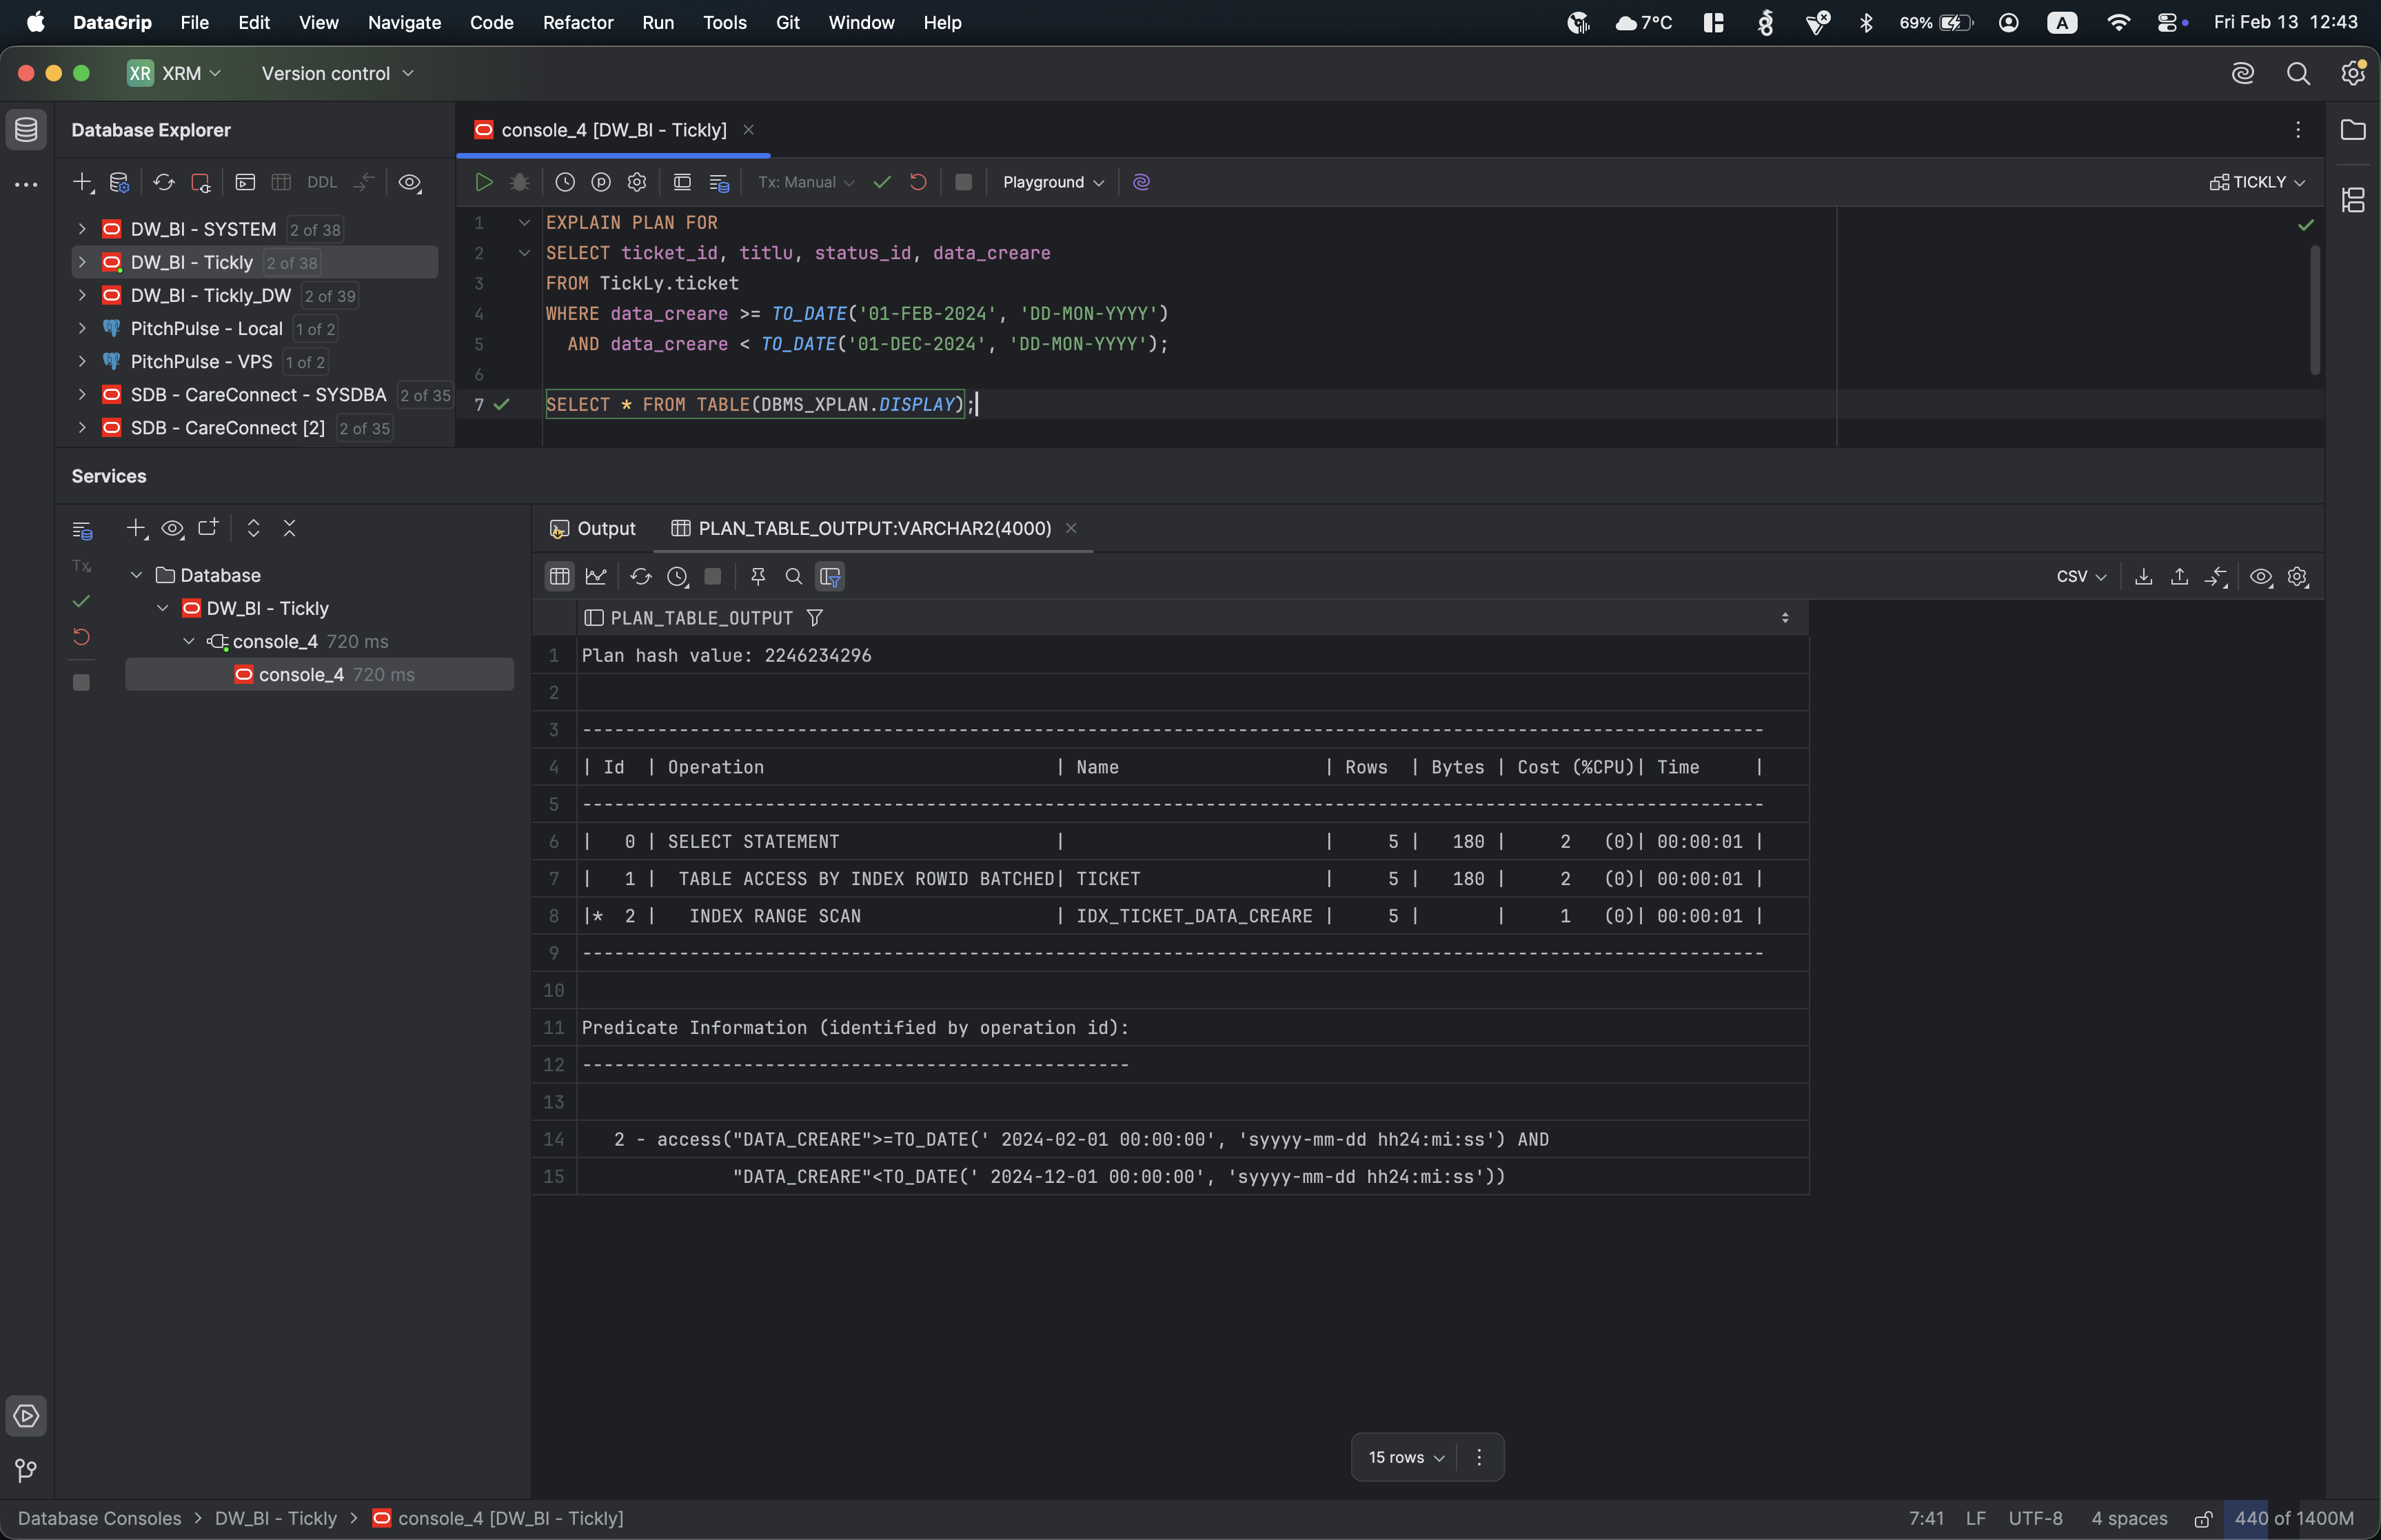
\includegraphics[width=\textwidth]{../../scripts/tests/assets/oltp_date_index_explain.png}
            \caption{Plan de execuție query 2}
            \label{fig:plan_executie_query_2}
        \end{subfigure}
        \caption{Analiză Query 2: Rezultat și Plan de interogare}
        \label{fig:analiza_query_2}
    \end{figure}

    \item \textbf{Depozit — indecși bitmap pe \texttt{fact\_ticket}}
    \begin{itemize}
        \item \textbf{3:} „Să se afișeze identificatorul din OLAP, cheia clientului și timpul de rezolvare (în ore) pentru tichetele care au un anumit status și/sau o anumită prioritate.”
    \end{itemize}

    \begin{verbatim}
        EXPLAIN PLAN FOR
        SELECT /*+ INDEX_COMBINE(f) */ f.fact_ticket_id, f.client_key, 
                                       f.timp_rezolvare_ore
        FROM TickLy_DW.fact_ticket f
        WHERE f.status_id = 3
        AND f.prioritate_id = 1;

        SELECT * FROM TABLE(DBMS_XPLAN.DISPLAY);
    \end{verbatim}

    \begin{figure}[H]
        \centering
        \begin{subfigure}[b]{0.48\textwidth}
            \centering
            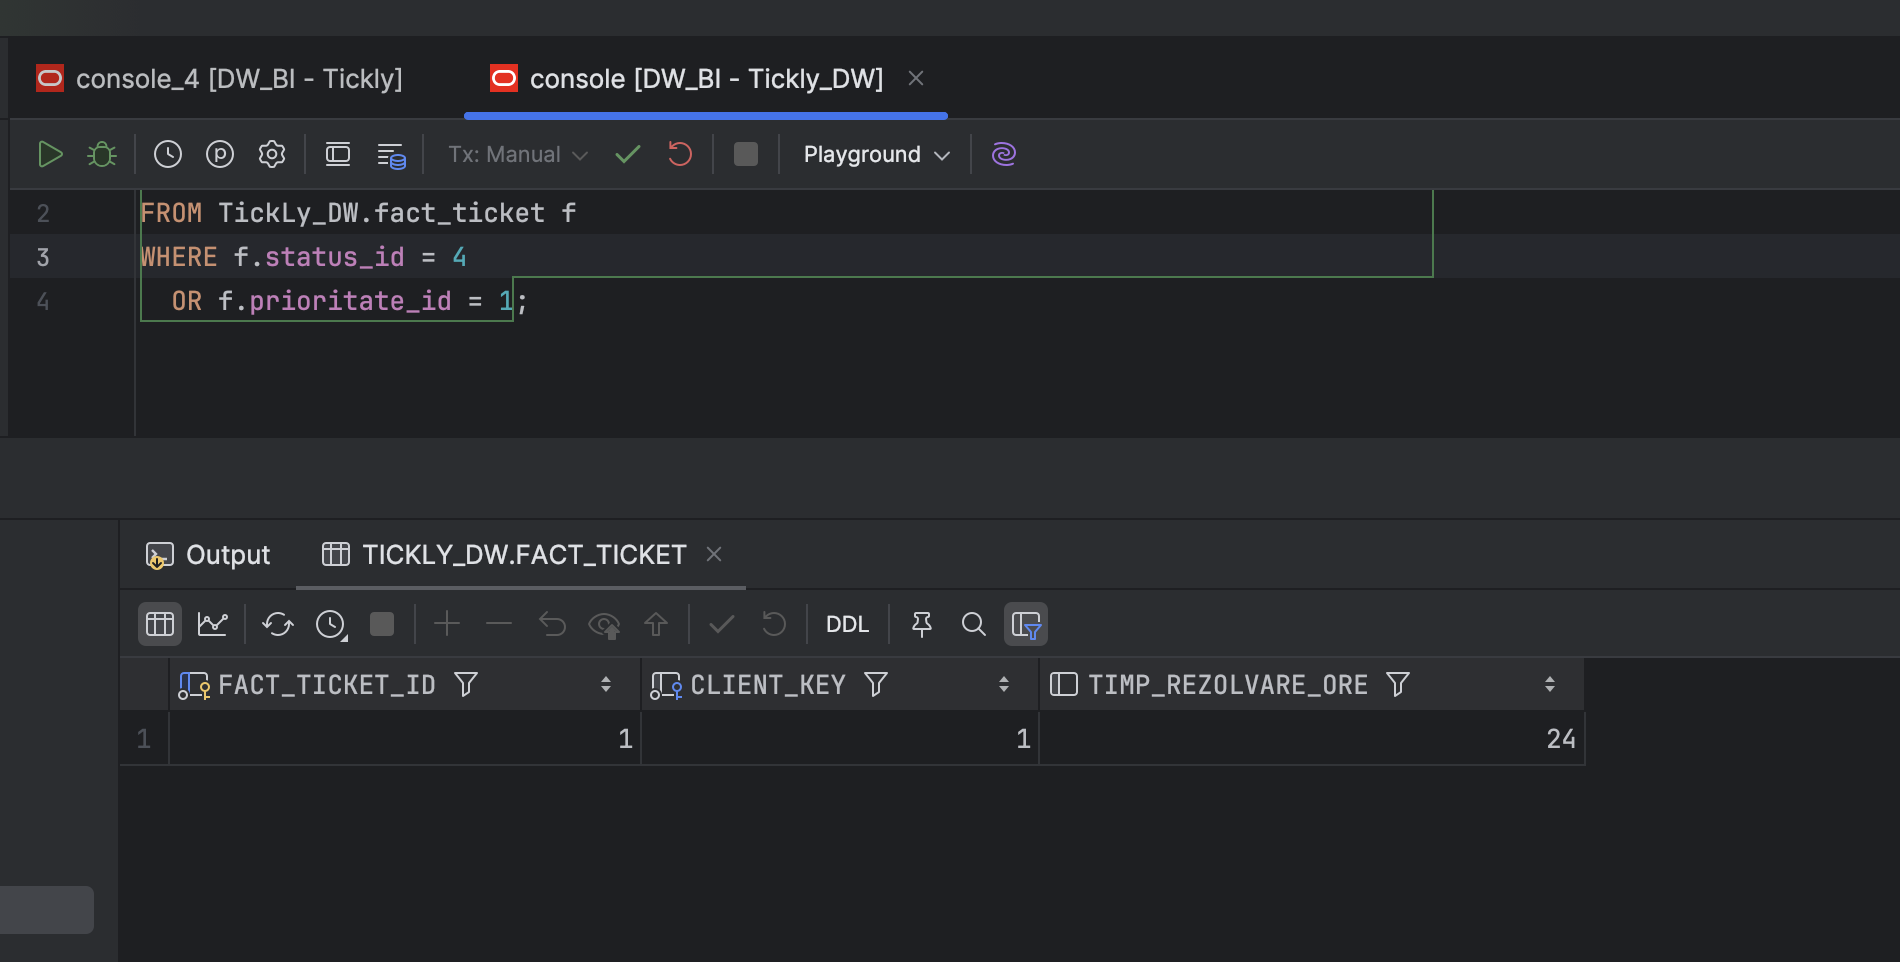
\includegraphics[width=\textwidth]{./assets/indexes/test_3.png}
            \caption{Rulare query 3}
            \label{fig:rulare_query_3}
        \end{subfigure}
        \hfill
        \begin{subfigure}[b]{0.48\textwidth}
            \centering
            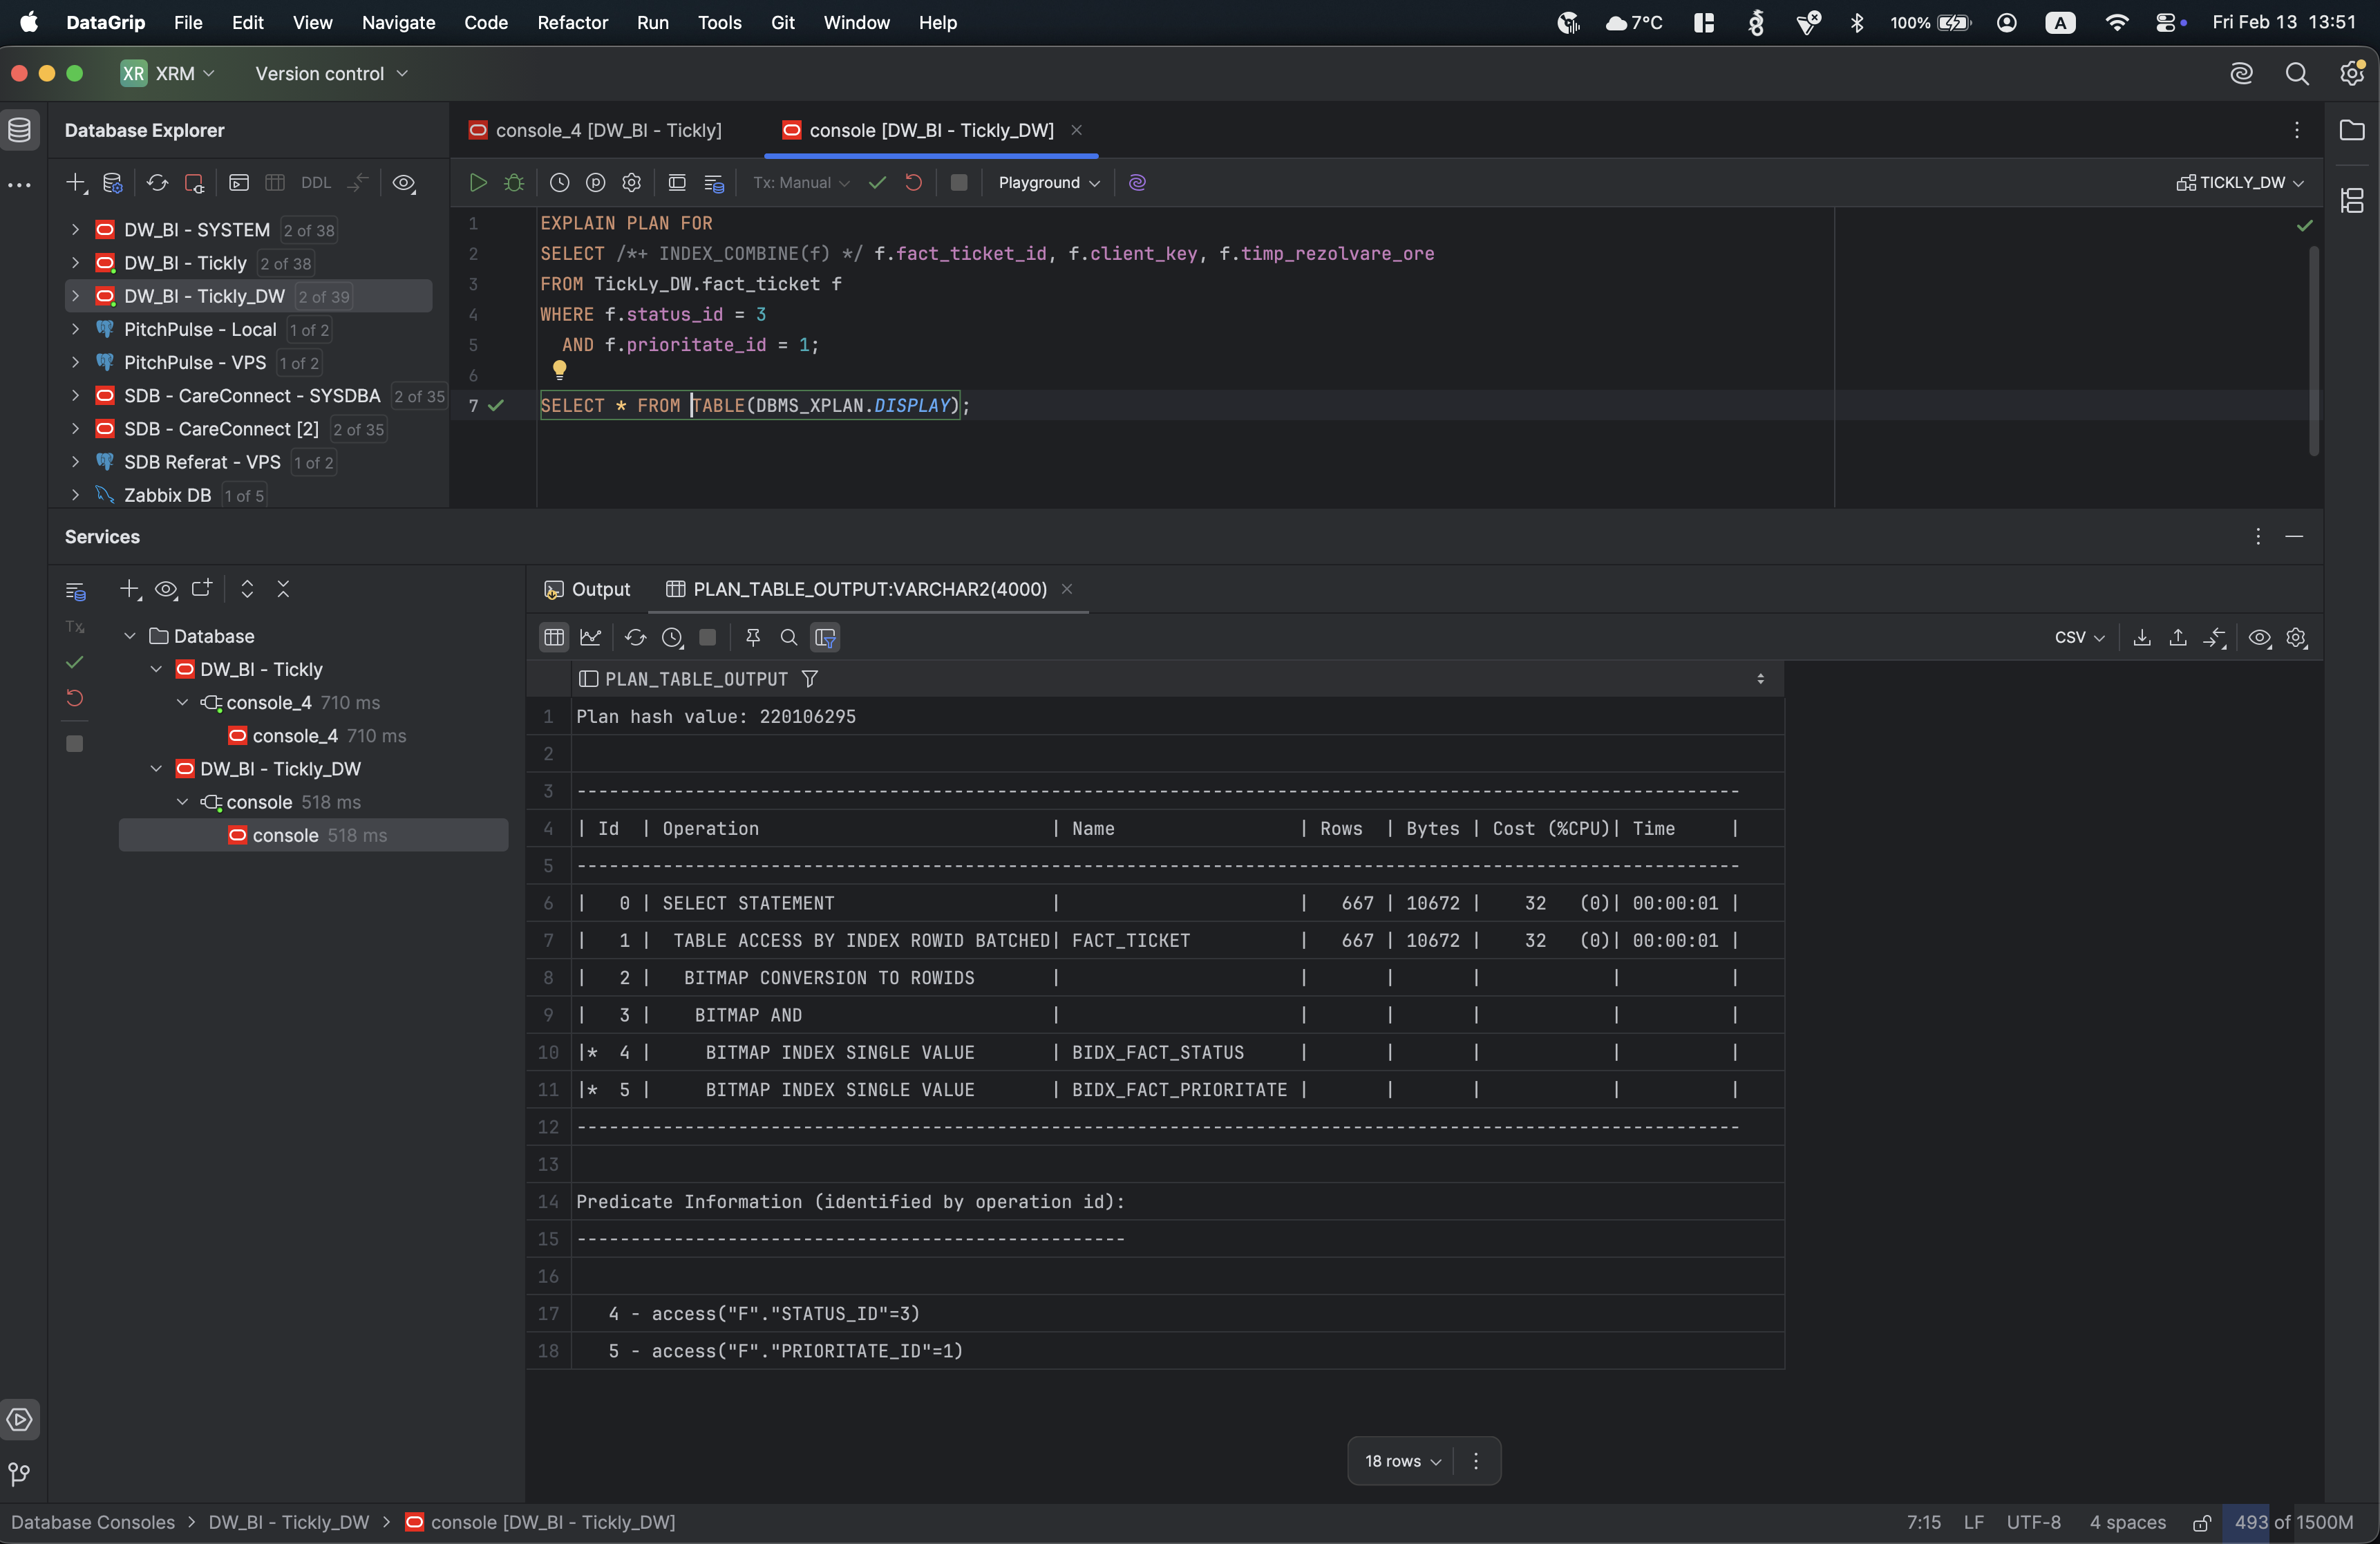
\includegraphics[width=\textwidth]{../../scripts/tests/assets/olap_status_prio_explain.png}
            \caption{Plan de execuție query 3}
            \label{fig:plan_executie_query_3}
        \end{subfigure}
        \caption{Analiză Query 3: Execuție și Plan de interogare (OLAP)}
        \label{fig:analiza_query_3}
    \end{figure}

\end{enumerate}
